\chapter{Working environment}
In section \ref{sec:vmclass} we introduced a classification of Virtual Machine systems.

The work presented in this thesis is restricted to same-ISA System Virtual Machines, where the Virtual Machine Monitor is a type 2 VMM.
In other words, we will deal with VMs that able to run an arbitrary OS compiled for the host ISA. The guest OS can in turn provide an 
execution environment for many user application.
Since the VMM is of type 2, it is implemented as a regular process in the host OS, and can make use of all the OS services.
We can therefore access the physical resource without requiring administrator previleges.

We also restrict our work to VMMs that make use of hardware-based virtualization, because the optimizations we will intrduce are
particularly effective in limiting the amount of VM switches between the host world and the guest world. Since these VM switches
are very expensive with hardware virtualization, the performance gain is significant.

While the assumptions made may appear restrictive, they are not at all. The class of VMMs that we consider is extremely 
common in the world of computing. They are used in datacenters and IT departments for server consolidation, 
application isolation, or to provide users/developers with zero-setup computing environments and other application in which it's
not important that the computing environment supported the VM has a different ISA from the host ISA.

\vspace{0.5cm}

Several VMM software belonging to the considered class are available. QEMU, VirtualBox, VMWare, Parallels, Windows
Hyper-V or Windows VirtualPC are among the most common examples of this kind of VMMs. These software tools are extremely widespread
and for this reason performance optimizations in these area are certainly useful.

This said, we have chosen the QEMU-KVM Virtual Machine Monitor for implementations and tests, although our optimizations are
relevant to the entire class of VMMs.

A GNU/Linux-based operating system (Archlinux) have been used on the host machine. The guest OS is generally Archlinux, but 
some tests have been performed with FreeBSD as a guest, too. Although Linux is a kernel and not a complete OS, in the following we 
will use  the expression ``Linux OS'' to actually mean ``GUN/Linux-based OS'', for the sake of simplicity.

\vspace{0.5cm}

Since our optimizations concern network performance, we had to choose a network device to work with. The \emph{e1000} class of 
network devices was chosen, since it is emulated by the vast majority of VMMs and supported by the main OSs (Windows, Linux, FreeBSD).


\section{QEMU features}
QEMU is a free, open source and multi-platform type 2 VMM, that makes use of dynamic translation to achieve good emulation performance.
QEMU-KVM is a QEMU branch that extends the original software to take advantage of hardware-based virtualization.
Whenever possible, QEMU-KVM uses hardware virtualization in order to execute guest code natively.
In the following we will use the terms QEMU and QEMU-KVM in an interchangeable manner.
At the date of this writing, the QEMU-KVM version number is 1.2.0, so we will refer to that version.

QEMU is a very flexible tool:
\begin{itemize}
    \item It supports process virtual machines: by means of dynamic translation it can execute on the host OS a single program compiled 
	  for an other ISA. This operating mode is called \emph{User mode emulation}.
	  
    \item It supports system virtual machines: by means of dynamic translation and hardware-assisted virtualization (when possible) it
	  can emulate full computer systems (including common peripherals), supporting unmodified operating systems. This operating
	  mode (which is the one we are interested in) is called \emph{Full system emulation}.
	  
    \item It supports various architectures, including  IA-32 (x86), x86-64, MIPS R4000, Sun's SPARC sun4m, Sun's SPARC sun4u,
	  ARM development boards (Integrator/CP and Versatile/PB), SH4 SHIX board, PowerPC,
	  ETRAX CRIS and MicroBlaze architectures.
	  
    \item It can emulate Symmetric Multiprocessing Systems (SMP), making use of all the CPUs that are present on the 
	  host system.
	  
    \item It is able to emulate various peripherals, such as hard disks, CD-ROM drives, network cards, audio interfaces, 
	  or USB devices.
	  
    \item Like similar hypervisors, it is able to provide its VM with network connectivity. The way this can be done will be
	  presented in section \ref{sec:qemunet}.
	  
    \item It does not normally require administrative rights to run. In our experiments administrative rights won't be
	  necessary.
\end{itemize}

QEMU is able to emulate the \emph{e1000} class of PCI network devices\footnote{To be more precise, the emulated hardware exposes
to the guest OS the PCI device ID of the 82540EM model.}, as well as other network devices (RTL8139C+, i8255x (PRO100), 
NE2000 (RTL8029), AMD PCNET II (Am79C7070a)).

In addition to that, QEMU support the \emph{Virtio} framework, that exposes a paravirtualized network device, virtio-net, intended 
to be used for high performance networking. The Virtio paravirtualized soution will be analized later.



\section{QEMU internal architecture}
In this section we will illustrate those details of QEMU implementation that are necessary to understand in order to reach our
goals.

\subsection{QEMU event-loop}
QEMU is an event-loop based software, and is implemented as a single-process multi-threaded application. 
One thread, referred to as \emph{IOThread}, executes the event-loop, waiting for new events to happen\footnote{This is 
implemented in \texttt{main-loop.c}}.
The waiting routine is a \texttt{select()} system call, which is not the most efficient choice on Unix-like systems
\footnote{ \texttt{poll()}, and espcially Linux \texttt{epoll()} or BSD \texttt{kqueue()} are more efficient},
but is more portable across different platforms.

\vspace{0.5cm}

The file descriptors associated with the \texttt{select()} can be associated to regular files, sockets, device files (such as TAP 
devices), or even special in-kernel objects, such as POSIX timers, signals and eventfds. These file descriptors are used by QEMU to let
the VM communicate with the host, and possibly with the rest of the Internet. In other words, they are used for performing the I/O 
operations requested by the VM. Of course the guest OS still performs I/O operations accessing I/O ports or memory-mapped I/O (MMIO) in 
his physical address space and is unaware of being emulated.

\vspace{0.5cm}

The QEMU core codebase offers to the QEMU developer an API that can be used to implement emulation of the devices.
The API also provides two useful abstractions: the QEMUTimer and the QEMUBH. 

QEMUTimers are a one-shot absolute timers, that can be 
used to execute a callback function at a certain point of time in the future. The callback is always executed by the IOThread, when it
recognizes that the deadline has been passed. The QEMUTimers are supported
by the Linux OS with a single one-shot relative POSIX timer\footnote{Similar mechanisms are used in other OS, or if POSIX timers are not
available under the Linux OS}, which is always (re)armed to expire - waking up the event-loop - at
the earliest deadline. The expire check for QEMUTimers is done at the end of each event-loop iteration, even if the event-loop was 
waken up for a reason different from the POSIX timer expiration. In the current implementation, moreover, every time the POSIX timer
is rearmed, the relative deadline is forced to be greater or equal that 250 $\mu$s\footnote{For more information about the QEMUTimer
interface and implementation, please refer to the file \texttt{qemu-timer.c} in the QEMU project root directory.}.

\vspace{0.5cm}

QEMUBH is the QEMU abstraction of the \emph{bottom half} concept, widely used in OS driver implementation. A QEMUBH can be seen as
a QEMUTimer that expires as soon as possible. In practice when a QEMUBH is scheduled, it notifies the event-loop, which in turn 
wakes up (or finishes the current iteration and begins another iteration) and execute all the callbacks of currently scheduled QEMUBHs.
Therefore the QEMUBH callbacks are always executed by the IOThread, similarly to the QEMUTimer callbacks\footnote{For more information
about the QEMUBH interface and implementation, please refer to the files \texttt{qemu-aio.h} and \texttt{async.c} in the QEMU project
root directory}. This feature is very important in terms of parallelism, as will be clear in the following chapters.

\subsection{VCPU Threads}
The IOThread, while executing the event-loop, handles all the interactions between the VM and the external world.
The guest code, however, is executed by one or more threads, that we will call \emph{VCPU threads}. In the current implementation QEMU
creates as many VCPU threads as the number of SMP processors specified by the users.
When using hardware-based virtualization (we made this assumption at the beginning of this chapter), a VCPU thread continuously
switch between the VM mode and the normal mode (see section \ref{sec:hbv}).

When the VCPU tries to execute an I/O operation - accessing I/O ports or MMIO - a VMExit happens. There could be other events
that cause a VMExit, but I/O operations are the type of events we are interested in. On a VMExit the VCPU stops executing guest
code and starts executing QEMU code, in order to handle - if is the case - the event that caused the VMExit.
When the event is handled, the VPCU executes e VMEnter and continues to run the guest code.

\vspace{0.5cm}

Since multiple threads are involved, and all of them - IOThread included - can access the shared structures used by the emulator
(e.g. the structures employed to implement the virtual devices), mutual exclusion is required. In the current implementation the
mutual exclusion is guaranteed by a single big-lock, called the \texttt{iothread lock}.

Therefore, on every VMExit a VCPU has to acquire the \texttt{iothread lock} before it can handle the event. After the event has been
handled, the VPCU thread release the \texttt{iothread lock} and execute a VMEnter instruction.
Similarly, the IOthread has to acquire the \texttt{iothread lock} every time it wakes up for event handling, and release the lock
only when the event-loop iteration terminates.

Putting all together, the figure \ref{fig:qemuthreads} depicts the QEMU thread scheme.

\begin{figure}[bt]
\centering
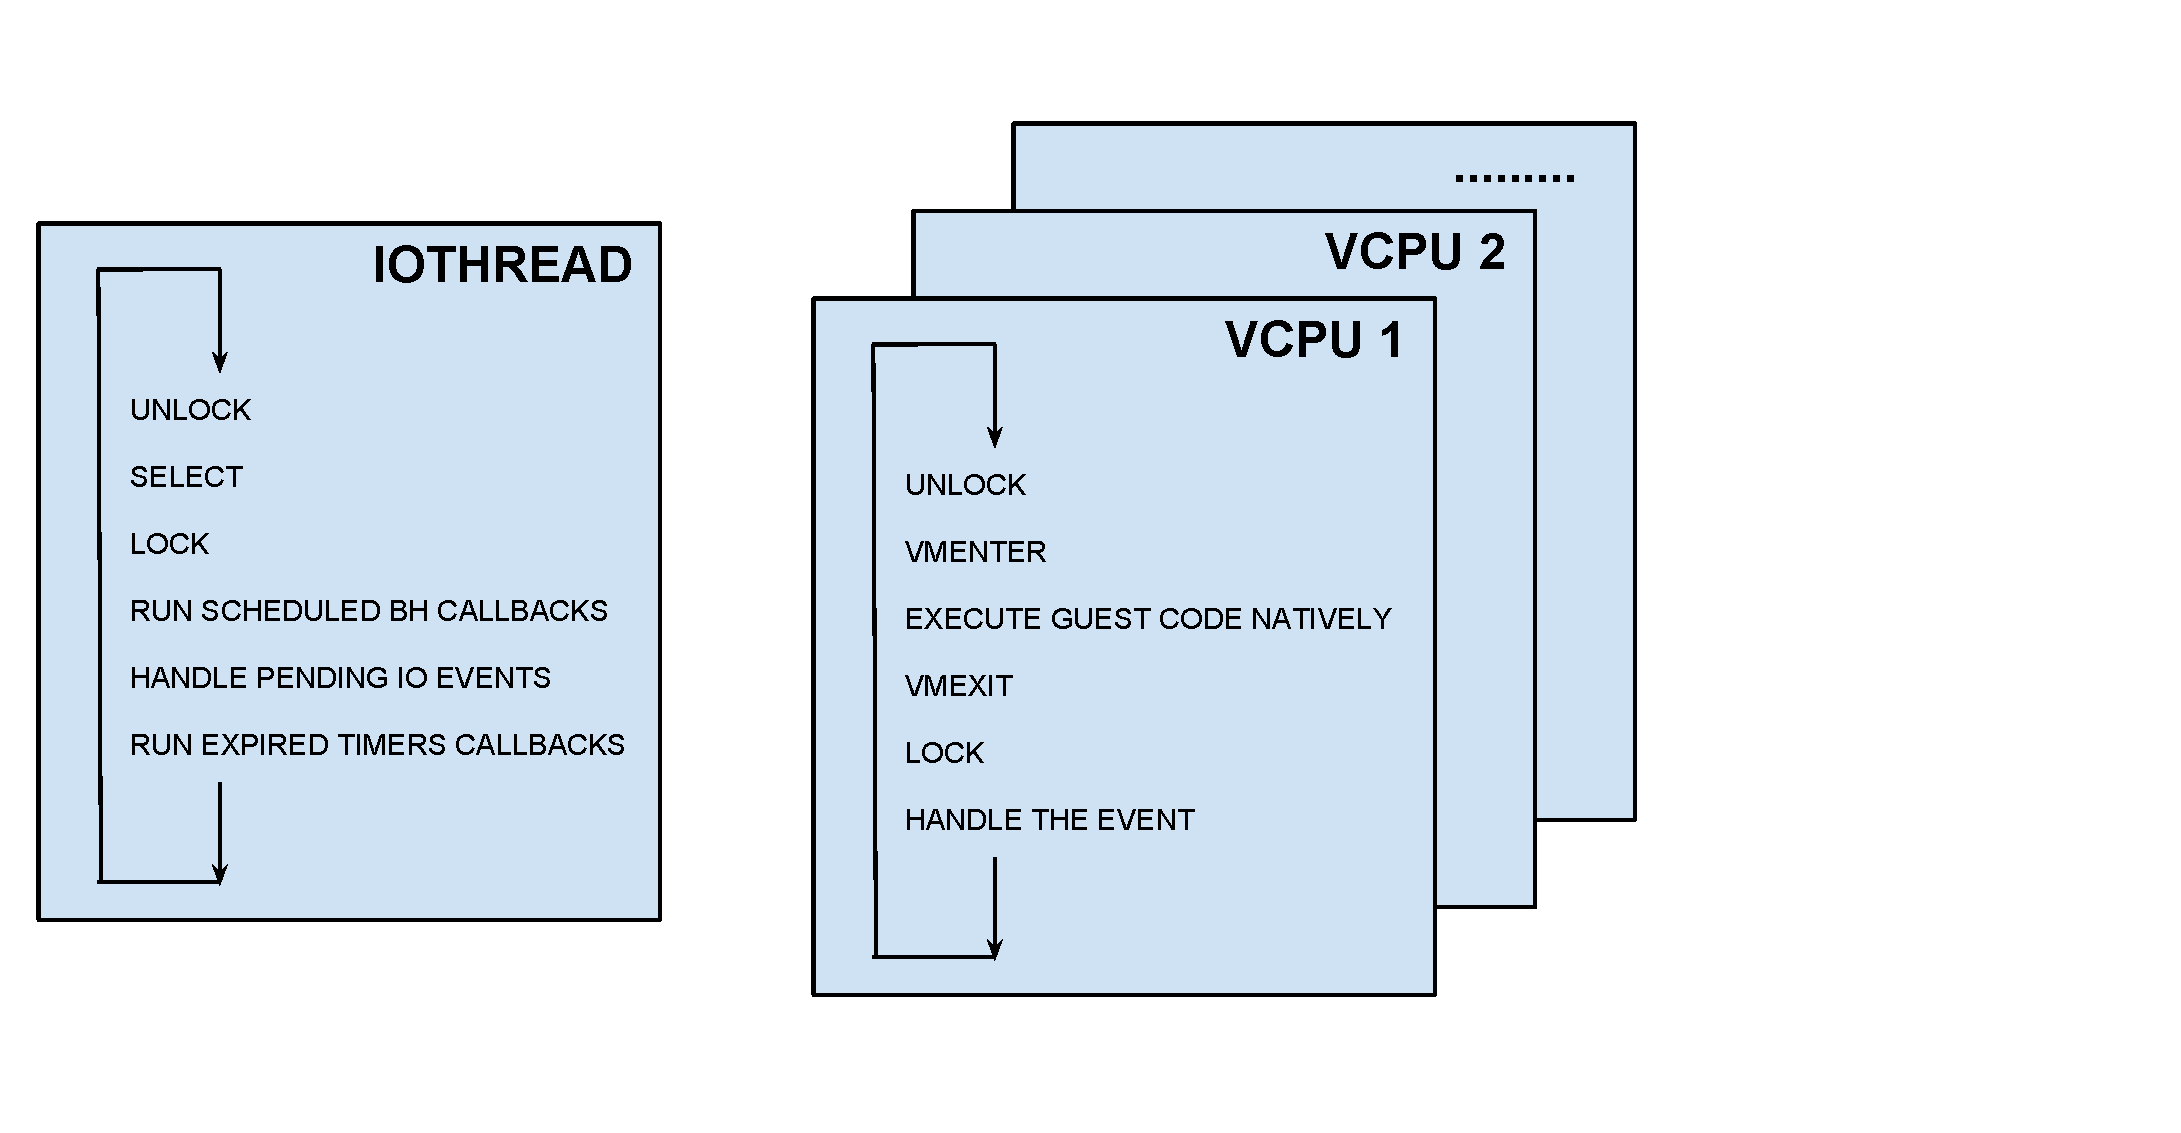
\includegraphics[scale = 0.45]{qemu-threads.pdf}
\caption{QEMU thread scheme.}
\label{fig:qemuthreads}
\end{figure}



\subsection{Networking architectures}
\label{sec:qemunet}
When running a VM it is of fundamental importance to make possible for the guest to communicate with the outside world using the
networking infrastructure, otherwise the VM itself would be an useless computing box.

Since the VM it's a software entity, however, it isn't connected to any real network. Therefore the hypervisor has to provide some
form of network infrastructure virtualization, so that the guest OS thinks its (virtual) network device is connected to a physical
network and can then exchange packets with the outside.

\vspace{0.5cm}

All the hypervisors cited previously (QEMU included) provide the VM administrator with a few virtual network infrastructure modes, 
so that she can choose the best way to connect her VM.

Three modes are commonly employed:
\begin{itemize}
    \item NAT mode. In this case the guest OS thinks to be physically connected to a completely fake LAN, entirely emulated inside the 
	  hypervisor. The VMM usually emulates a DHCP server, a DNS server and a gateway router, so that the guest OS can configure
	  its network interfaces and its routing tables
	  and communicate with the outside world. When the guest sends a TCP/UDP packet on the fake LAN, the VMM intercepts the packet,
	  performs address translation (NAT) turning the guest source IP (the guest IP) into the host IP and sends the packet towards
	  its destination using the host OS services (thus the host OS routing tables). The inverse translation is performed when
	  receiving a packet.
	  
	  In this way the VM is easily provided with Internet connectivity, but it's not visible form the outside
	  and cannot communicate with other VMs present on the same host.
	  In QEMU this mode is called \emph{Usermode networking}.

    \item Host-only mode. Also in this case the guest OS thinks to be physically connected to a LAN. The LAN is emulated
	  by means of a software bridge (that emulates a layer-2 network switch), and the VM is connected to a port of the bridge.
	  More VMs can be connected to the same bridge, making inter-VM communication possible. The software bridge can be internally
	  implemented in the hypervisor, or can be an external software bridge.
	  
	  Whit QEMU this mode can be set up on a Linux host using the in-kernel bridging and TAP interfaces. Each VM is assigned a TAP
	  interface where can write/read ethernet frames, and all the TAPs are bridged together to the in-kernel bridge.
	  In this way a frame sent by the guest is written by QEMU to its associated TAP and is therefore routed by the bridge
	  to the correct destination TAP. The receiving QEMU process can then read the frame from the TAP and push it to its VM.
	  In this case no DHCP or DNS server is emulated, and you have to configure yourself the network of each VM\footnote{The 
	  configuration can be static or you can run a DHCP server on one of the VMs connected to the bridge.}.
	  Since the software bridge itself has its separate network interface, also the host can communicate on the LAN.
	  
    \item Bridged mode. This mode is an extension of the host-only mode. The only difference is that a physical host network interface
	  is also bridged to the VMs LAN. Since the physical interface becomes a bridge port, the host can access the physical network
	  through the software bridge interface.
	  In this way the host can share its connectivity with all the VM connected to the software bridge. If the physical interface
	  is connected to a LAN, with this configuration the VMs LAN appears to be part of the physical LAN.
	  
\end{itemize}
	
Clearly the NAT mode is not interesting with respect to our goals, since it is only intended to be a way the VM can easily obtain
Internet connectivity, and it's not intended to be a flexible networking mode. Instead we will consider host-only mode, since we
are intersted in optimizing the communication performance between two VMs on the same software bridge or between a VM and the host
bridge interface. In this work it would make no sense considering to bridge also the host physical interfaces (bridged mode), 
because we optimizing performance of physical network adapter it's not among our goals.


\subsection{Network frontend and backend}
In order to implement a specific networking architecture, the QEMU implementation includes a degree o separation, namely an interface,
between the piece of code that emulates the network device and the code that provides access to the chosen networking model.
This is done because the two subsystems are completely independent, and you can easily combine every virtual network device with
every networking access mode.

Using the QEMU terminology, the network device emulation is also called \emph{network frontend}, and the networking access mode is
called \emph{network backend}. 

\vspace{0.5cm}

In our case the network frontend is ``e1000'' and it's implemented within the file hw/e1000.c (in the QEMU project root directory).
This source file is the only one that contains code which is specific to the e1000 class of networking devices, exporting to the rest 
of the system the same interface exported by the other network devices.

The network backend can be
\begin{itemize}
    \item ``user'', which implements Usermode networking.
    \item ``tap'', which is an implementation of host-only/bridged networking that relies on TAP devices and in-kernel bridges.
    \item other implementations of host-only/bridged networking that use a different software bridge solutions, maybe in conjunction
	  with TAPs and in-kernel bridges. The ``VALE'' backend (\cite{ref:vale}) is an example of high performance alternative 
	  implementation of the host-only/bridged networking access mode.
\end{itemize}

\vspace{0.5cm}

Frontend and backend can be seen as two peers connected to each other that are able to exchange ethernet frames. Each peer exports a 
\texttt{receive} method that accepts an ethernet frame as argument\footnote{The ethernet frame frame can be specified with an address 
and a length, or with a scatter-gather array.}. That method will be invoked whenever the other peer wants to send a frame.

In this way, when a frontend wants to send a frame to the network, it invokes the \texttt{send\_packet} function provided by the QEMU
networking API, that will invoke the \texttt{receive} method exported by the backend. The backend \texttt{receive} method will push the
frame onto the network, in a way that is specific to the backend itself.

On the other direction, when the backend gets a frame from the network, it invokes the \texttt{send\_packet} function, that will in turn
invoke the \texttt{receive} method exported by the frontend. This method will push the frame into the guest system in a way that is
specific to the network device model.

The frontend-backend communication is depicted in figure \ref{fig:frontback}.

\begin{figure}[bt]
\centering
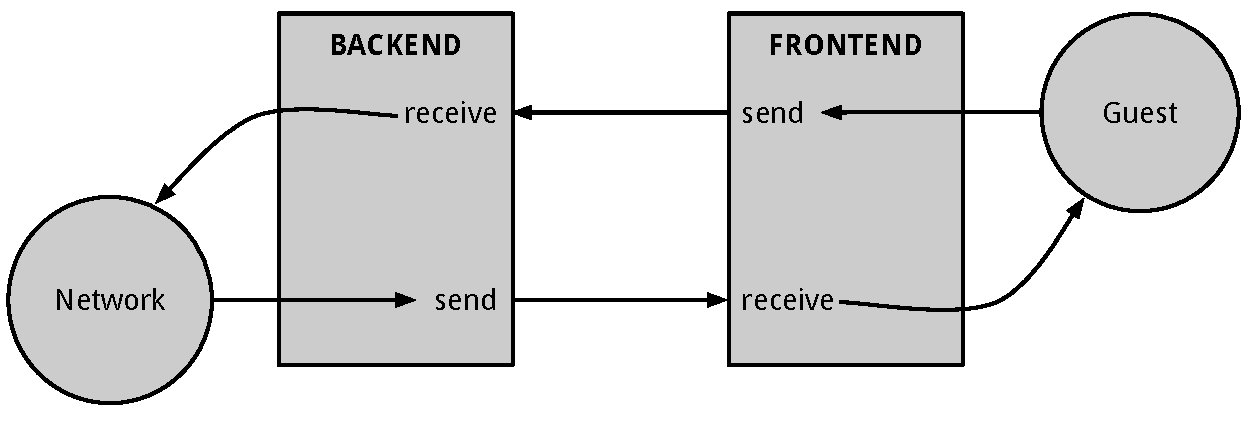
\includegraphics[scale = 0.60]{frontend-backend.pdf}
\caption{Interface between network frontend and network backend.}
\label{fig:frontback}
\end{figure}



\section{The e1000 class of network adapters}
In this section we will illustrate some features and some details about the inner working of an e1000 ethernet network adapter.
Once again, we will only describe those aspects that are relevant to our goals.
The complete specification can be found in %cite Intel.

\vspace{0.5cm}

Since the network communication is extremely important in the IT world, the market constantly pushes hardware vendors to produce high
performance, low-power, fully featured flexible network devices.

As a result, modern network devices are very complex. To get an idea of this complexity, one can observe that a device can implement 
more then a hundred of software-visible registers. The complexity is the price to pay in order to get high flexibity and several useful
features. Flexibility helps the IT administrator to tune the device parameters in order to find the right tradeoff between performance and 
power consumption, throughput and latency, and the like.
The rich set of features the device come with helps to adapt the device to different usage patterns and allows for performance 
optimizations (expecially for TCP/IP traffic) when offloading capabilities are present.

Hardware offloading features are supported by virtually every recent network adapter.
The most common feature are
\begin{itemize}
    \item Checksumming offload. When this feature is present, the device computes in hardware the checksums required by the main Internet 
	  protocols, such as IP, TCP and UDP. This saves the OS to do this work in software, which could be very expensive, expecially 
	  with checksums that are computed also on the payload and not only on the protocol header (e.g. TCP and UDP checksums).
	  
    \item TCP Segmentation Offload. When this feature is present, the device is able to do the TCP segmentation in hardware, splitting
	  a TCP segment over multiple ethernet frames. The segmentation is necessary because the real MTU of a TCP connection is almost
	  never greater than 1500 bytes (the ethernet original MTU), but the TCP window is commonly greater than that value. The OS
	  is then forced to do the splitting. With the feature present, however, the OS can send to the device driver a frame containing a 
	  TCP segment which is greater than the MTU\footnote{Up to 64KB with the Linux kernel.}. The device driver can pass the packet to
	  the device that perform the segmentation in hardware and send multiple ethernet frames.
	  Apart from the obvious speed-up obtained because the operation is done in hardware rather then in software, this mechanisms has 
	  an important positive side effect. The network overhead necessary to traverse the TCP/IP stack is suffered only once, for a
	  big TCP packet, instead of once for each MTU-sized fragment. This clearly amortize the kernel per-packet overhead.
	  
    \item Scatter-gather capability. When this feature is present, the device is able to send a frame that is stored in multiple non
	  contiguous fragments in the machine physical memory. Therefore the OS is not forced to linearize (gather) the fragments,
	  avoiding the copy overhead. This is useful specially when the OS wants to send large packets. In other words the device is 
	  gather-capable.
\end{itemize}
The e1000 devices have this three features.


\subsection{Data interface with the driver}
Being high performance devices, modern network adapters rely on Direct Memory Access (DMA) operations and interrupts.

When the device driver wants to send an ethernet frame through the adapter, it has to tell the device where the frame is stored
in physical memory and how long it is\footnote{When dealing with fragmented frames, the driver has to specify somehow a scatter-gather
array.}. Once the device knows where the frame is, it can directly access the physical memory\footnote{In this example we assume
there isn't any IOMMU.} and send it on the wire. More commonly, the frame is DMA'ed into an internal buffer for further processing before
being sent on the wire, but this is just a detail.

When the adapter receives a frame from the wire, it has to store it in the machine physical memory. For this reason, the device driver
has to tell the adapter where it can store incoming frames, before the frames actually came. If the adapter doesn't know how to put
incoming frames, it cannot accept them.

\vspace{0.5cm}

It is clear that there must be a well-defined interface between the driver and the device. This interface is known as \emph{ring}.
A ring is a circular array of \emph{descriptors} that are used to exchange address/length information\footnote{Being an array a ring is a 
contiguous zone in the physical memory.}. A network adapter have at least two rings.
The first one is the \emph{TX ring} and it is used with outgoing frames, whereas the second is the \emph{RX ring}, and it is used with
incoming frames. Network adapter can have multiple TX/RX rings with possibly different policies and priorities, so that one can
do some traffic engineering.

However, the e1000 adapter model emulated by QEMU has one TX ring and one RX ring. The array length, namely the number of descriptors,
can be decided by the driver to a certain extent. In e1000 it must be a power of two and not more than 4096.


\subsubsection{TX ring}
The e1000 TX ring is an array of $N$ TX descriptors. Each TX descriptor is 16 bytes long and contains the address (in physical memory) and the
length of a frame (or a frame fragment) that is going to be sent or that has already been sent. The descriptor contains also flags that
can be used to specify options, and status bits. 

Two index registers are implemented for the synchronization between the driver and the adapter:
The TDT register (Transmit Descriptor Tail) and the TDH register (Transmit Descriptor Head). These are \emph{index} registers since
their value are array indexes with respect to the TX ring descriptors array.

At the start-up, TDT and TDH are initialized by the driver to the same value, usually 0. When the driver wants to send a new frame,
it writes the physical address and the length of the frame in the TX descriptor pointed by the TDT register and then increments the TDT
register itself. Since the descriptor array is circular, the TDT must be set adequately.

When the adapter recognizes that TDH is different by TDT, is knows that there are new frames to transmit, and start processing the
descriptor pointed by TDH, sending on the wire the frame pointed by the descriptor (if is the case), and then increments the TDH register.
The adapter stops the processing only when TDH has the same content as TDT has. A write access to the TDT register is therefore the
way the device driver notifies the adapter that there are new frames ready to be sent.

When the driver increments the TDT, the descriptor previously pointed (the one that has just been written) is committed to the hardware,
and the hardware owns it until the decriptor is processed.

Therefore, in each moment the ring is partitioned in two contiguous parts: The descriptor owned by the hardware, which are waiting
to be sent on the wire, and the descriptors owned by software, which are free to be used by the driver to commit new frames.

In order to prevent the index registers to wrap around, the driver should not never use a TX descriptor if this is the very last free
TX descriptor. This happens when TDT is shuch that incrementing it circularly would cause TDT == TDH. When the TX ring is in this
state (TX ring full), the driver should stop transmitting. The transmission can be enabled again when the hardware process some descriptors,
incrementing TDH.

The figure \ref{fig:txring} depicts the TX ring with its index registers.

\begin{figure}[bt]
\centering
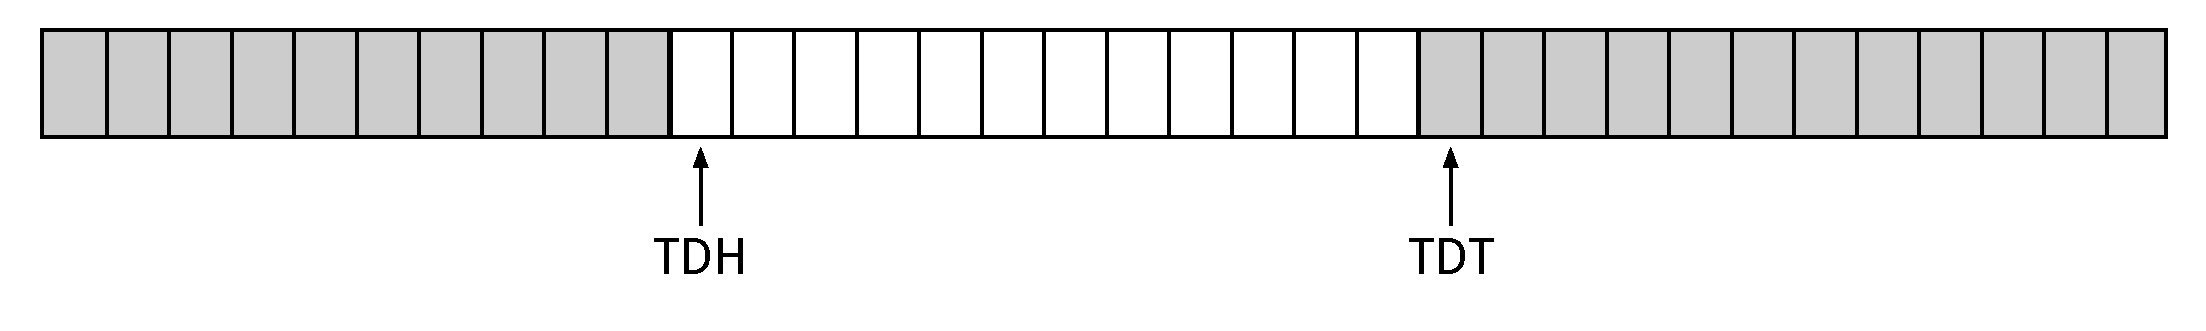
\includegraphics[scale = 0.35]{tx-ring.pdf}
\caption{The e1000 TX ring with its index registers. The grey area contains software-owned descriptors, while the white area
	contains hardware-owned descriptors.}
\label{fig:txring}
\end{figure}


\subsubsection{RX ring}
The e1000 RX ring is an array of $N$ RX descriptors. Each RX descriptor is 16 bytes long and contains the address (in physical 
memory) and the length of a frame that has been received by the adapter, or only the address of a memory location that can be
used by the adapter to store an incoming frame. The descriptor contains also flags that can be used to specify options and status bits.
Two index registers are implemented for the synchronization between the driver and the adapter:
The RDT register (Receive Descriptor Tail) and the RDH register (Receive Descriptor Head). These are \emph{index} registers since
their value are array indexes with respect to the RX ring descriptors array.

At the start-up, the driver initializes RDH and RDT to 0. At this point, the adapter still doesn't know of any memory buffer where it
can store incoming frames, so it cannot receive anything.
To give the hardware memory buffers to work with, the driver puts the physical address of a memory buffer\footnote{How the memory 
buffer is allocated depends on the OS and on how the driver is implemented.} in the RX descriptor pointed by RDT and increments 
RDT circularly. Writing to the length field of the RX descriptor is useless, since this value is not used by the device. It's important to note
that the size of the memory buffer must be greater or equal then the maximum frame length, since we cannot know in advance how long
a future frame is going to be.

A write access to the RDT register is therefore the way the device driver notifies the adapter that there are new memory buffers ready
to be used to store incoming frames.

If the adapter sees that RDH is different by RDT, it recognizes to have memory buffers available, and starts accepting incoming frames.
When a new frame arrives from the wire, the adapter fetches the RX descriptor pointed by the RDH register, copies the frame to the address
contained in the RX descriptor, writes back the length of the received frame to the RX descriptor itself and increments the RDH register
circularly.
At this point, if programmed to do so, the device would normally sent an interrupt (see section \ref{sec:e1000int}, in order to tell
the driver there are new received frames ready to be pushed to the kernel network stack.

When the driver increments the RDT, the descriptor previously pointed (the one that has just been written) is committed to the hardware,
and the hardware owns it until the decriptor is used.

Therefore, in each moment the ring is partitioned in two contiguous parts: The descriptor owned by the hardware, which can be
used to store new incoming frames, and the descriptors owned by software, which are unused or point to received frames ready to
be pushed to the network stack.

Similarly to what happens the TX ring, in order to prevent the register indexes to wrap around, the driver should never increment the RDT
register if the increment would cause RDT == RDH. When this situation happens (full RX ring) the driver should stop giving memory buffers to
the adapter. When new frame are received, the hardware increments RDH, and so it is possible to restart.

The interrupt routine should then push the arrived frames to the kernel and provide the adapter with more memory buffers (incrementing
the RDT), otherwise the adapter cannot accept more incoming frames.

A common strategy is to try to keep the RX ring always full. In order to do this, at the startup
the driver writes $N-1$ RX descriptor with the address of $N-1$ memory buffers, and set RDT to $N-1$, so that the ring is full-
Every time an interrupt arrives, the interrupt routine pushes the received frames to the kernel and replenish the ring, making it full again.
This strategy avoid situations in which the adapter is forced to reject incoming frames because it has no memory buffers available.

The figure \ref{fig:rxring} depicts the RX ring with its index registers.

\begin{figure}[bt]
\centering
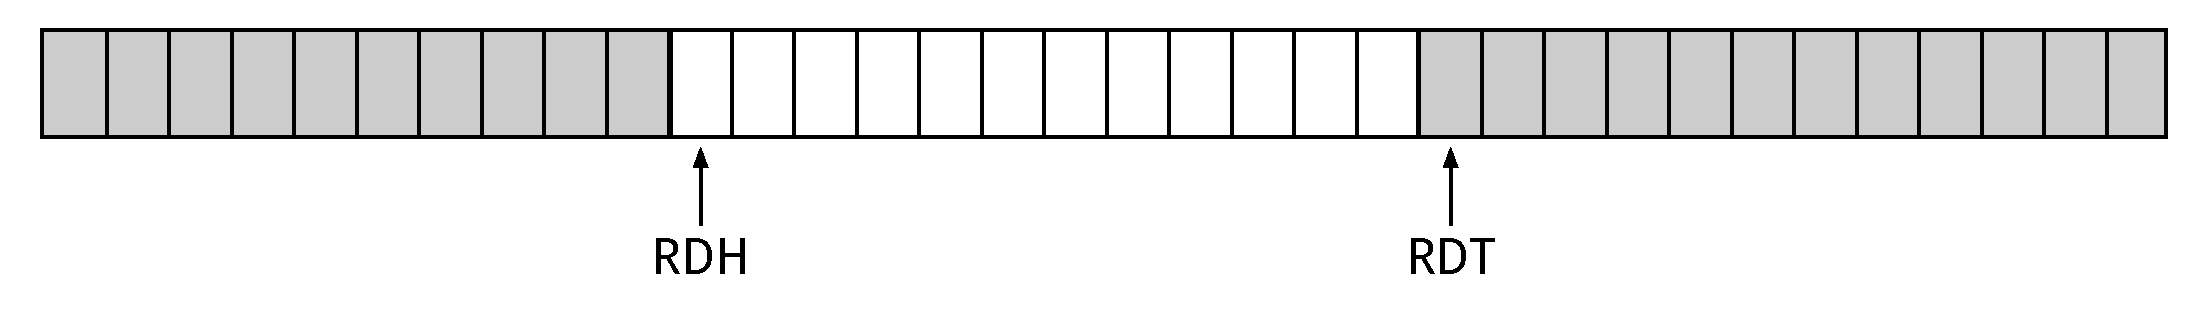
\includegraphics[scale = 0.35]{rx-ring.pdf}
\caption{The e1000 RX ring with its index registers. The grey area contains software-owned descriptors, while the white area
	contains hardware-owned descriptors.}
\label{fig:rxring}
\end{figure}


\subsection{Interrupts generation}
\label{sec:e1000int}
The e1000 network adapter can generate interrupts for different reasons.

We are interested in two types of interrupt:
\begin{itemize}
    \item TX interrupts: these interrupts are generated when the transmission of one ore more hardware-owned frames completes. Each TX 
	  descriptor has
	  a bit flag (Report Status, RS) that can be set to specify if the harware should send an interrupt as soon as the transmission 
	  of the associated
	  frame is complete. In every case an interrupt is always sent when the TX ring becames empty (TDH == TDT).
	  The interrupt routine, depending on the OS and the driver implementation, may execute cleanup operations on the descriptors 
	  that have been processed and mark them as free to be used to commit new frame to the adapter.
	      
    \item RX interrupts: these interrupts are generated after the hardware has received (and stored in physical memory) an incoming frame, 
	  in order to notify the driver that can send the frame to the kernel network stack. When the frame is sent to the kernel, it will
	  find the right way to its destination, that can be anything (trash included). Assuming the destination is a user process,
	  what the OS does is just to append the packet to a queue associated to the receiving socket. At this point the sleeping user
	  process is notified and can be scheduled to complete the read operation from the socket queue.
\end{itemize}

There is a big concern when dealing with RX interrupts. If the device doesn't limit them, they act as a source of uncontrolled load for the 
CPU.
The receiving machine, in fact, is forced to serve incoming RX interrupts even if the RX interrupt rate is very high. Since we are
dealing with high performance devices, we must be able to receive up to 1 Mpps (or even more).
The overhead involved in interrupt handling is generally quite high, and so each interrupts has a fixed cost that must be paid before
doing useful work, such as push the received frame to the network stack and let the receiver process actually receive it.

If each packet receive generated an interrupt, we would have to handle up to 1000000 interrupts per seconds, which something that would
completely stall our machine.
When the interrupt rate is too high, in fact, the machine spends almost all the time serving interrupts\footnote{The interrupt handling is
by its nature an high priority task with respect to normal process execution.}, and there is no time left for other things to happen,
e.g. for user processes to read the received packets. This is a quite bad situation, because the CPU is 100\% utilized, but the machine,
on the whole, cannot do any useful work.

The situation could be slightly better if the machine has more than one CPU, but still it's not good for the CPU servicing the interrupts
to spend too much time in interrupt handling overhead.

\vscpae{0.5cm}

Cleary, this problem can only be solved if the device somehow collapses RX interrupts, raising an interrupt every batch of received
frames, let's say 100 frames per batch, and not every single frame. In this way the interrupt rate is 100 time lower, and the
interrupt overhead cost is amortized over 100 frames.
In every case the device must guarantee that a RX interrupt is eventually sent after a period of inactivity, even if it is still waiting
for a 100-frames batch to be completed, because the device cannot know when the next frames are going to come.

These and similar mechanisms are know as \emph{interrupt mitigation} or \emph{interrupt moderation}, since they tries to moderate the
interrupt rate.

Interrupt moderations is commonly applied also to TX interrupts (or to all the interrupts in general). The TX interrupt rate can be
controlled because the driver can control (and limit) the TX rate. Neverthless it is convenient for the driver to take advantage of
the interrupt-rate-limiting hardware capabilities rather than implement a similar feature in software\footnote{With e1000, an TX 
interrupt moderation mechanism could be implemented using the RS bit.}.

\vspace{0.5cm}

The e1000 class of network adapters implements two interrupt moderation mechanisms.




%In our case the \emph{e1000} device is implemented through a single source file\footnote{hw/e1000.c in the QEMU project root directory}.
%A small part of this code contains declarations and routines necessary to register and initialize/uninitialize a new PCI Ethernet 
%device within the rest of the emulator. In this way one or more instances of the e1000 network device can be included by the QEMU users
%when launching QEMU\footnote{This is done through the \texttt{device} option. E.g. \texttt{qemu-kvm -device e1000 ...} }.
